%%%%%%%%%%%%%%%%%%%%%%%%%%%%%%%%%%%%%%%%%%%%%%%%%%%%%%%%%%%%
%%
\newcommand{\resistorRow}[3]{%
    \noindent
    \begin{minipage}[c]{0.49\textwidth}
        \includegraphics[width=5cm]{#1} 
    \end{minipage}%
    \hfill
    \begin{minipage}[c]{0.5\textwidth}
        \large
        Widerstandswert: \underline{\hspace{0.2cm} #2 \hspace{0.2cm}} \\[0.3cm]
        Toleranz: \hspace{1.3cm} \underline{\hspace{0.2cm} #3 \hspace{0.2cm}}
    \end{minipage}
    
    \vspace{1cm} % Abstand zur nächsten Reihe
}
%%
%%%%%%%%%%%%%%%%%%%%%%%%%%%%%%%%%%%%%%%%%%%%%%%%%%%%%%%%%%%%
%% AUFGABE 4
%%%%%%%%%%%%%%%%%%%%%%%%%%%%%%%%%%%%%%%%%%%%%%%%%%%%%%%%%%%%

\newpage
\section{Wertebestimmung von Widerstand und Kondensator}
Ziel dieser Aufgabe ist die Entwicklung zweier Programme zur Bestimmung elektrischer Größen. Das erste Programm dient der Ermittlung eines Widerstandswertes, das zweite der Berechnung einer Kapazität.

\subsection{Vorbereitung}

\subsubsection{Widerstandsbestimmung}

\resistorRow{resistor1.png}{\SI{47}{\kilo\ohm}}{$\pm \SI{5}{\percent}$}
\resistorRow{resistor2.png}{\SI{3.9}{\mega\ohm}}{$\pm \SI{5}{\percent}$}
\resistorRow{resistor3.png}{\SI{6.8}{\kilo\ohm}}{$\pm \SI{10}{\percent}$}

\subsubsection{Spannungsteiler}

\paragraph{a)} Die Spannung teilt sich am Spannungsteiler im Verhältnis der Widerstände auf.
\[
    U_{R1} = U_e - U_a = \SI{5}{\volt} - \SI{3}{\volt} = \SI{2}{\volt}
\]
Das Verhältnis der Widerstände $R_1 : R_2$ entspricht dem Verhältnis der Spannungen $U_{R1} : U_a$, also \textbf{2:3}. Berechnung von $R_2$ mit $R_1 = \SI{10}{\kilo\ohm}$:
\begin{align*}
    \frac{R_1}{R_2} &= \frac{U_{R1}}{U_a} \implies R_2 = R_1 \cdot \frac{U_a}{U_{R1}} \\
    R_2 &= \SI{10}{\kilo\ohm} \cdot \frac{\SI{3}{\volt}}{\SI{2}{\volt}} = \SI{15}{\kilo\ohm} 
\end{align*}

\paragraph{b)} Der Widerstand $R_2$ wird durch $R_x$ ersetzt. Die neue Ausgangsspannung beträgt $U_a = \SI{1}{\volt}$.
\[
    U_{R1} = \SI{5}{\volt} - \SI{1}{\volt} = \SI{4}{\volt}
\]
Berechnung von $R_x$:
\begin{align*}
    R_x &= R_1 \cdot \frac{U_a}{U_{R1}} = \SI{10}{\kilo\ohm} \cdot \frac{\SI{1}{\volt}}{\SI{4}{\volt}} = \SI{2.5}{\kilo\ohm} \\
\end{align*}

\subsubsection{Kondensatorladung}

\paragraph{a)} Die Spannung am Kondensator folgt der Ladefunktion:
\[
u_c(t) = U_q \cdot \left(1 - e^{-\frac{t}{\tau}}\right)
\]
Es ist bekannt, dass der Kondensator nach der Zeitkonstante $\tau = R \cdot C$ circa \SI{63}{\percent} der Endspannung erreicht hat ($1 - e^{-1} \approx 0.63$). Da nach $t = \SI{100}{\milli\second}$ genau dieser Wert erreicht ist, gilt:
\[
\tau = \SI{100}{\milli\second}
\]
Daraus lässt sich die Kapazität $C$ berechnen:
\[
    \tau = R \cdot C \implies C = \frac{\tau}{R} = \frac{\SI{1.1}{\second}}{\SI{10}{\kilo\ohm}} = \SI{0.00001}{\farad} = \SI{10}{\micro\farad}
\]

\paragraph{b)} Der Kondensator gilt als vollständig geladen (Spannung $> 99\,\%$), wenn eine Zeit von ca. $5 \cdot \tau$ vergangen ist ($1 - e^{-5} \approx 0.993$). Die Ladedauer beträgt somit:
\[
    t_{\text{voll}} \approx 5 \cdot \tau = 5 \cdot \SI{100}{\milli\second} = \SI{500}{\milli\second}
\]

\subsection{Durchführung}

\tikzset{ameter/.style={rmeterwa, t=A}}
\tikzset{vmeter/.style={rmeterwa, t=V}}

\begin{figure}[h]
    \begin{subfigure}[t]{0.25\textwidth}
    \centering
    \begin{circuitikz}
        \draw (0,0) node[vcc]{\SI{5}{\volt}}
            to[R=$R_\text{REF}$] ++(0,-2) coordinate (k1)
            to[R=$R_x$] ++(0,-2) node[ground]{};
        \draw (k1) to[short, *-o] ++(1,0) node[above]{IO-PIN};
    \end{circuitikz}
    \caption{Widerstandsmessung mit Arduino}
    \end{subfigure}\hfill
    \begin{subfigure}[t]{0.25\textwidth}
    \centering
    \begin{circuitikz}
        \draw (0,0) node[vcc]{\SI{5}{\volt}}
            to[R=$R_\text{REF}$] ++(0,-2) coordinate (k1)
            to[C=$C_x$] ++(0,-2) node[ground]{};
        \draw (k1) to[short, *-o] ++(1,0) node[above]{IO-PIN};
    \end{circuitikz}
    \caption{Kapazitätsmessung mit Arduino}
    \end{subfigure}\hfill
    \begin{subfigure}[t]{0.25\textwidth}
    \centering
    \begin{circuitikz}
        \draw (0,0) node[vcc]{\SI{5}{\volt}}
            to[R=$R_\text{REF}$] ++(0,-2) coordinate (k1)
            to[R=$R_x$, *-] ++(0,-2) node[ground]{};
        \draw (k1) -- ++(1.5,0)
            to[vmeter, v^=$U_x$] ++(0,-2) node[ground]{};
    \end{circuitikz}
    \caption{Spannungsmessung}
    \end{subfigure}\hfill
    \begin{subfigure}[t]{0.25\textwidth}
    \centering
    \begin{circuitikz}
        \draw (0,0) node[vcc]{\SI{5}{\volt}}
            to[R=$R_\text{REF}$] ++(0,-1)
            to[R=$R_x$] ++(0,-1)
            to[ameter, i_=$I_x$] ++(0,-2) node[ground]{};
    \end{circuitikz}
    \caption{Strommessung}
    \end{subfigure}
    \caption{Messschaltung zur Strom und Spannungsmessung eines Widerstands.}\label{fig:ui-mess}
\end{figure}

Die für die Durchführung benötigten Bauteile sind in \autoref{tab:bom4} aufgeführt.

\begin{table}[h]
    \centering
    \caption{Stückliste}\label{tab:bom4}
    \begin{tabularx}{\textwidth}{XXXX}
        \toprule
        \textbf{Bez.} & \textbf{Bauteil} & \textbf{Wert} & \textbf{Stückzahl} \\ \midrule
        $R_\text{REF}$ & Widerstand & \SI{10}{\kilo\ohm} & 1 \\ 
        $R_x$ & Widerstand & unbekannt & 4 \\ 
        $C_x$ & Kondensator & unbekannt & 3 \\ \bottomrule
    \end{tabularx}
\end{table}

\subsubsection{Aufbau am Steckbrett Widerstandsmessung}

Vor dem Aufbau wurde eine Prototyp-Schaltung in Tinker-CAD\footnote{\href{https://www.tinkercad.com/things/6dP6bOFcvVJ-4-widerstandsmessung?sharecode=cloxrV9fQVUj9Cfl4C-4CEYhAw4g13SRQi1Q5vM9bJg}{Tinker CAD Share Link}} aufgebaut und emuliert, um die Durchführung am Steckbrett zu erleichtern.

\begin{figure}[h]
    \centering
    
\includegraphics[width=\textwidth]{tinkercad4res.png}
    \caption{Planung des Aufbaus in TinkerCAD.}
\end{figure}

Im Anschluss wurde die Schaltung am Steckbrett aufgebaut.

\begin{figure}[h]
    \centering
    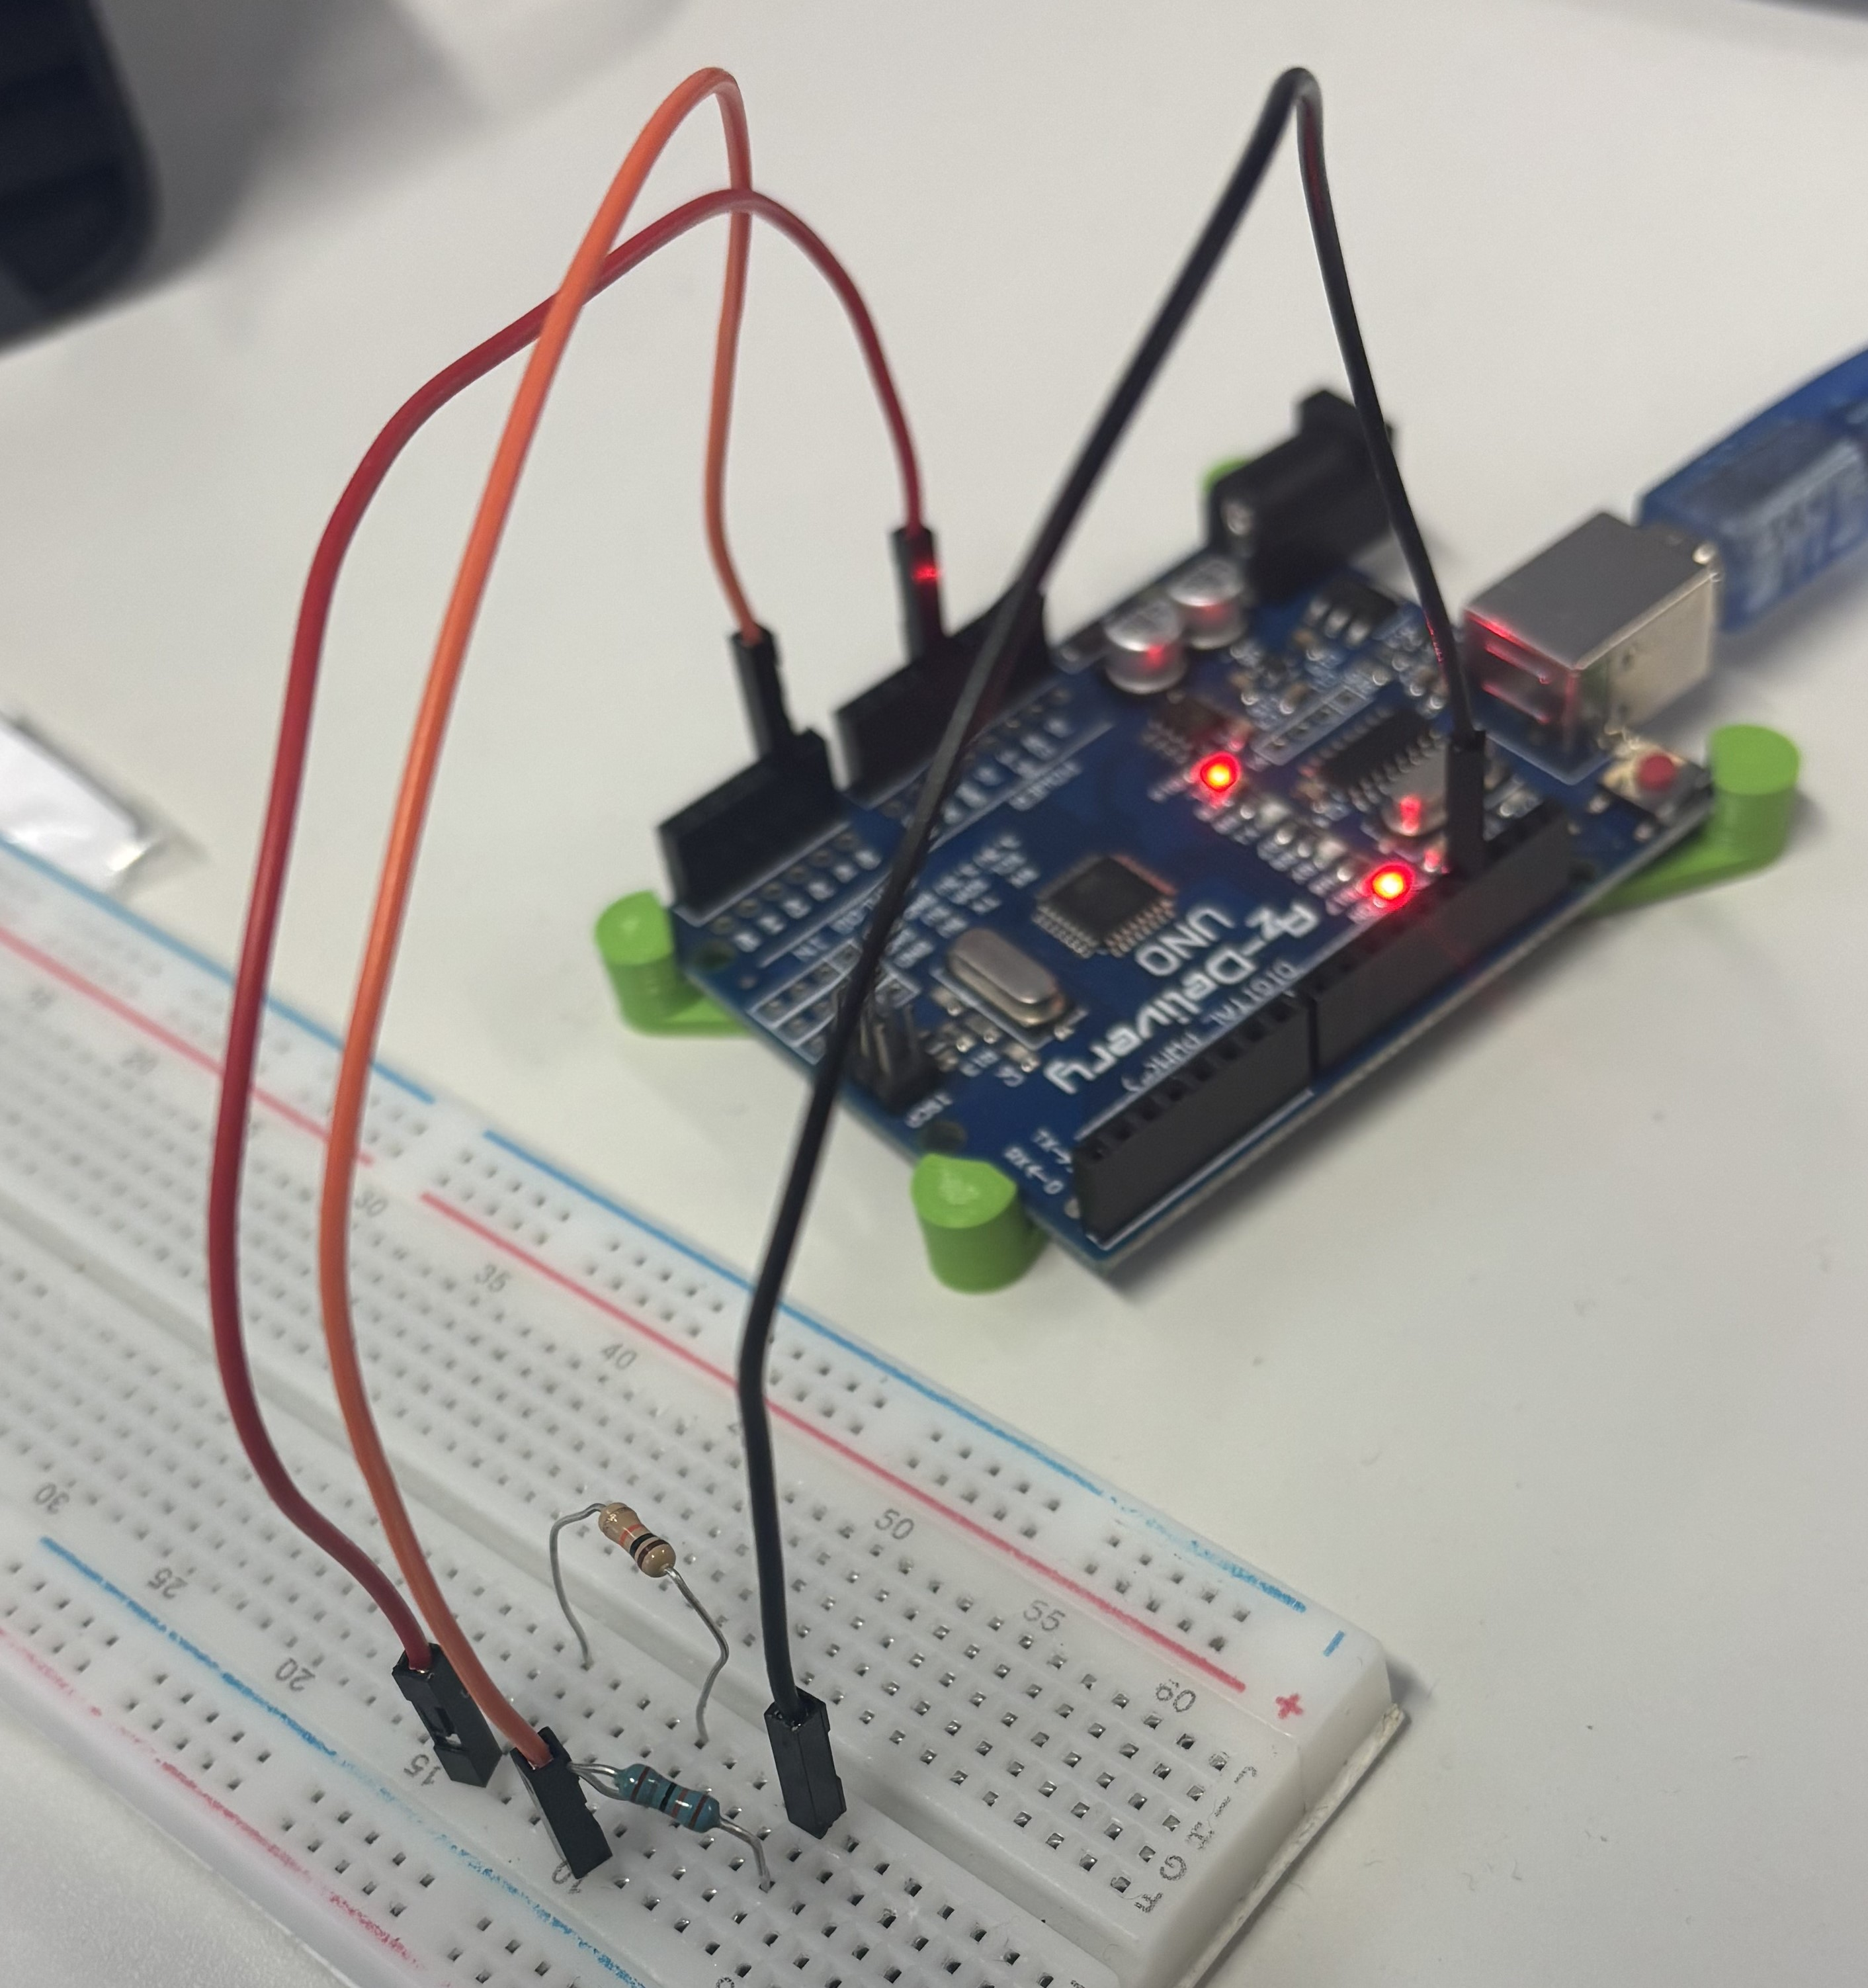
\includegraphics[height=5cm]{latex/images/fotos/4_a.JPEG}
    \caption{Verdrahtung am Steckbrett.}
\end{figure}

\subsubsection{Aufbau am Steckbrett Kapazitätsmessung}

Vor dem Aufbau wurde eine Prototyp-Schaltung in Tinker-CAD\footnote{\href{https://www.tinkercad.com/things/84XtVuCZHAm-4-kapazitatsmessung?sharecode=4kCbAaRwm3v1nCWt6jAq8217Vbh7pe0KWzrzvLyUI0Q}{Tinker CAD Share Link}} aufgebaut und emuliert, um die Durchführung am Steckbrett zu erleichtern.

\begin{figure}[h]
    \centering
    
\includegraphics[width=\textwidth]{tinkercad4cap.png}
    \caption{Planung des Aufbaus in TinkerCAD.}
\end{figure}

Im Anschluss wurde die Schaltung am Steckbrett aufgebaut.

\begin{figure}[h]
    \centering
    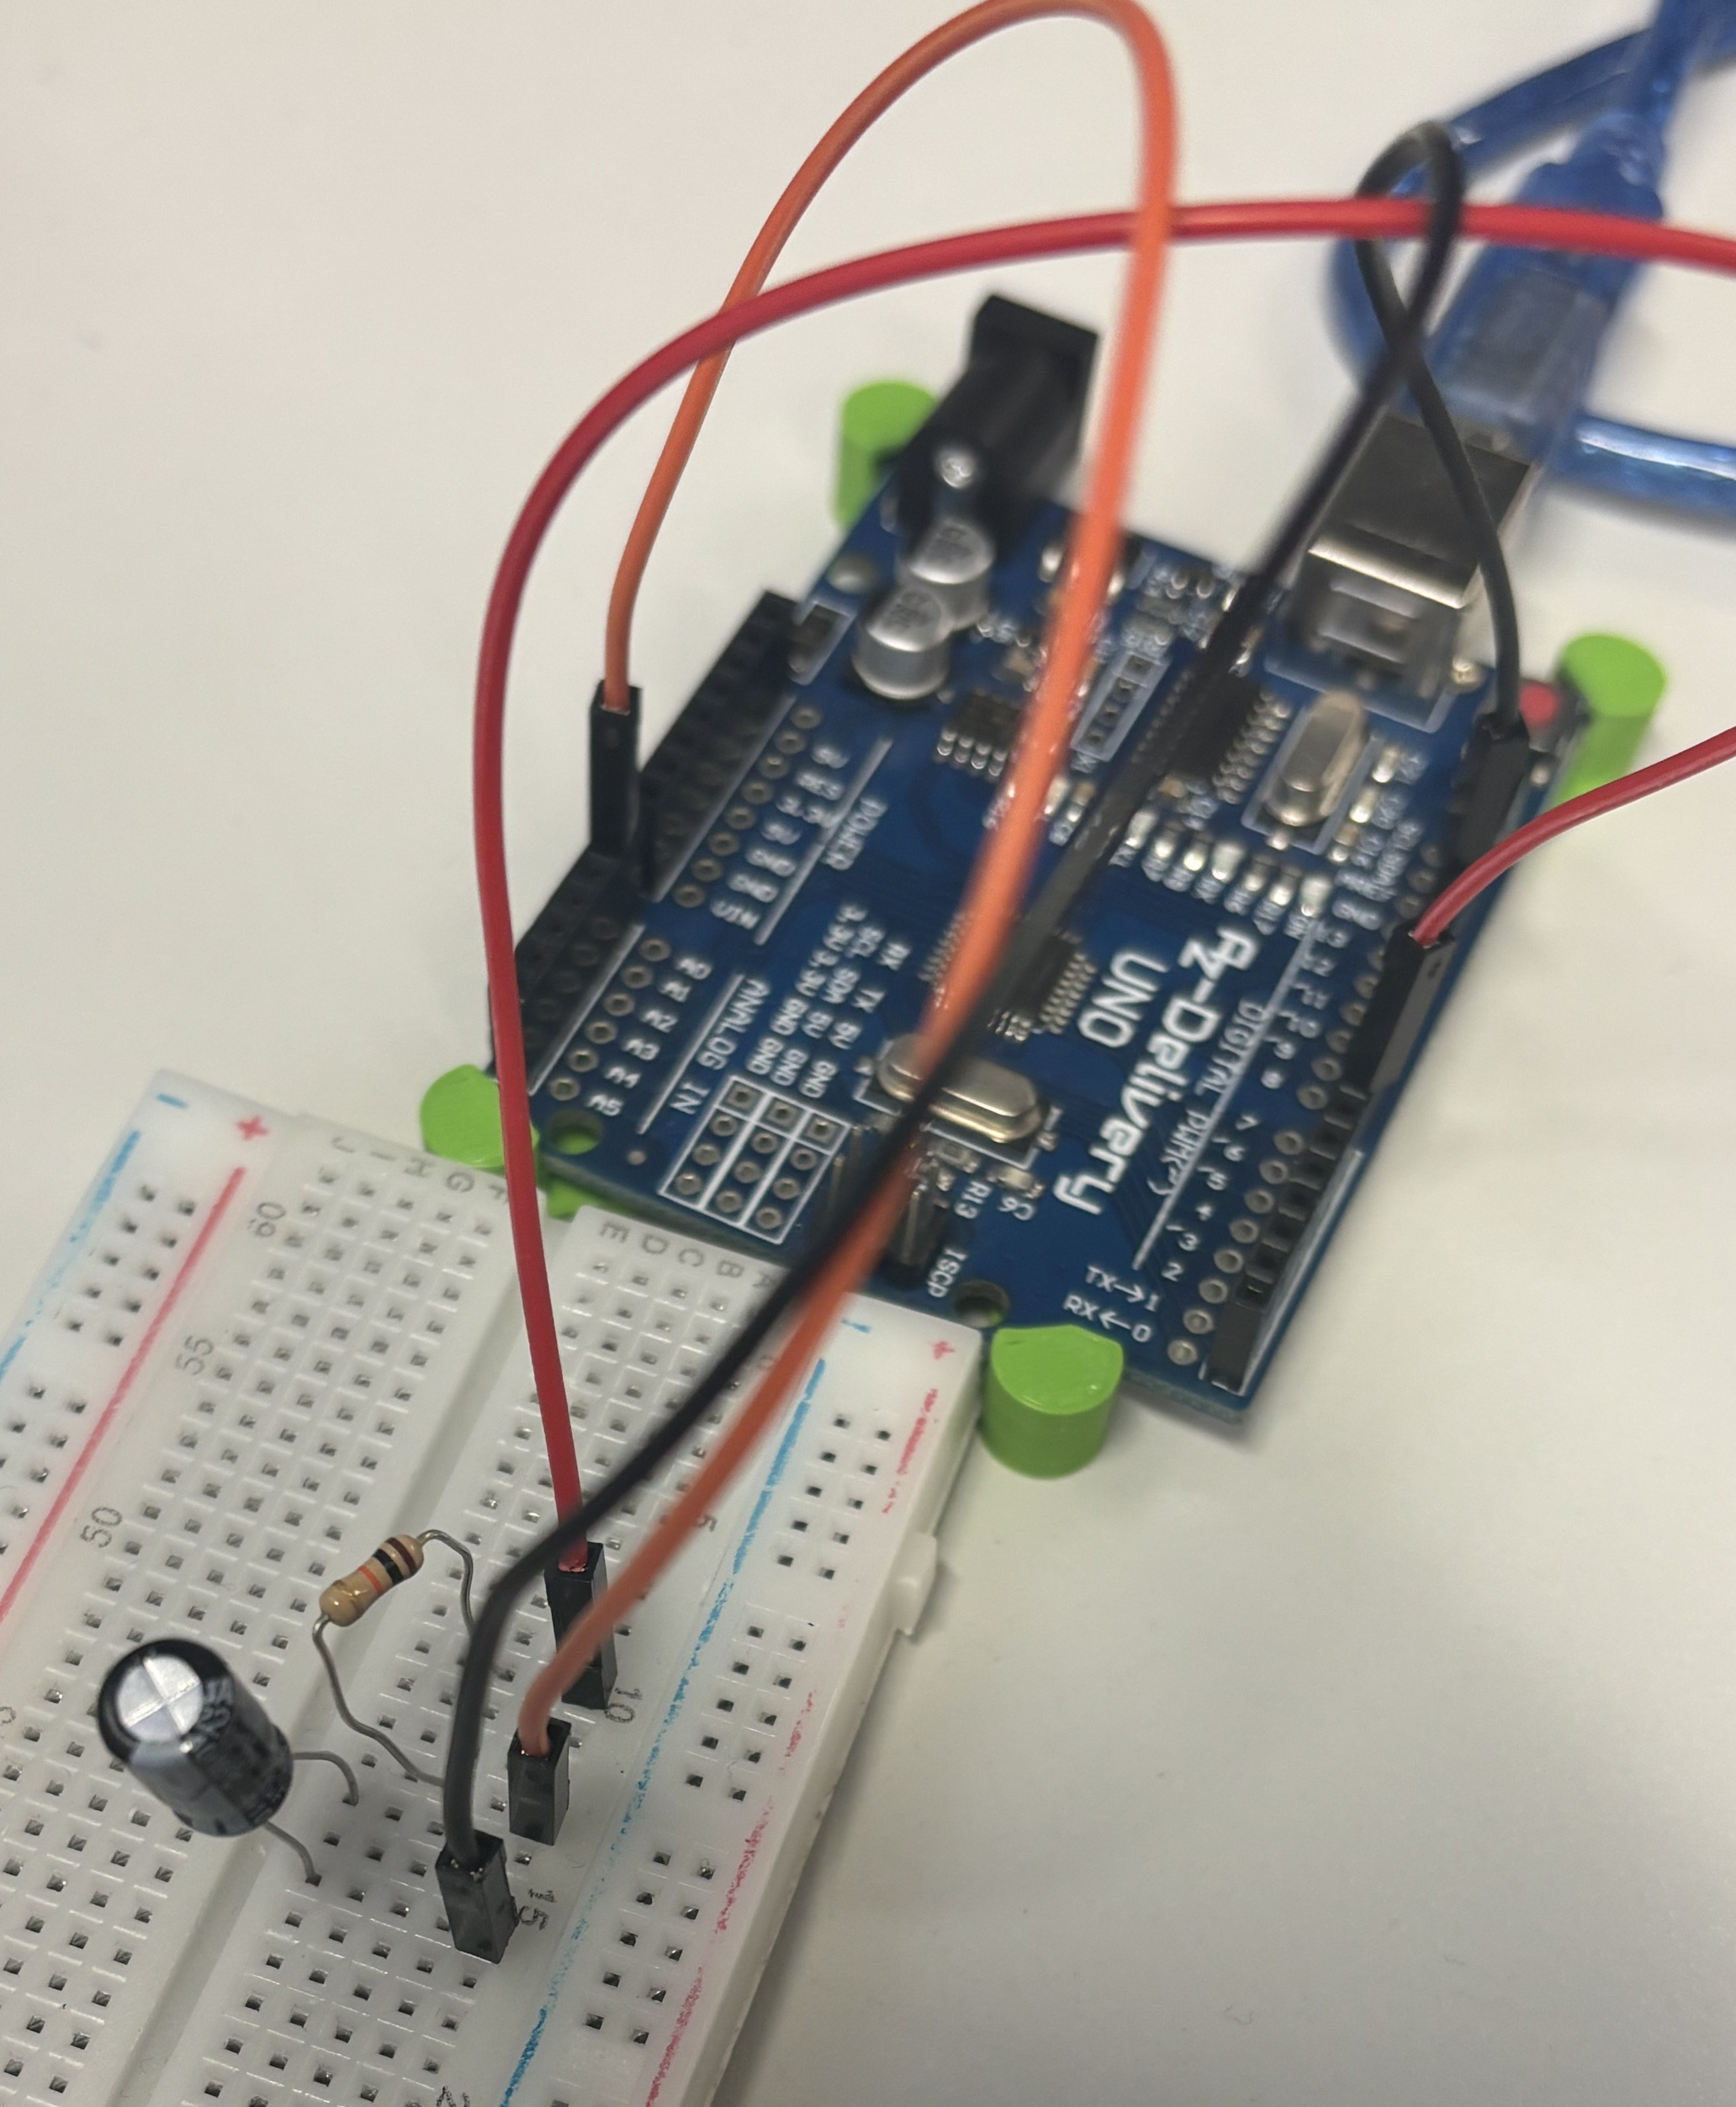
\includegraphics[height=5cm]{latex/images/fotos/4_b.JPEG}
    \caption{Verdrahtung am Steckbrett.}
\end{figure}

\newpage
\subsubsection{Implementierung der Widerstandsmessung}

\lstinputlisting[
    lastline=3,
    caption={Globale Variablen und Definitionen}
]{../04-Widerstand/res/res.ino}

\lstinputlisting[
    firstline=5,
    caption={Setup und Loop}
]{../04-Widerstand/res/res.ino}


\subsubsection{Messmethode}



\newpage
\subsection{Ergebnisse}

\subsubsection{Widerstand 1}

\paragraph{Ohmmeter} gemessen: \SI{100.3}{\ohm}

\paragraph{Farbcode} Der Widerstand weist 5 Ringe mit folgenden Farben auf:

\begin{tabularx}{\textwidth}{Y|Y|Y|Y|Y}
    \color{white}\textbf{Braun}\cellcolor{brown} &
    \color{white}\textbf{Schwarz}\cellcolor{black} &
    \color{white}\textbf{Schwarz}\cellcolor{black} &
    \color{white}\textbf{Schwarz}\cellcolor{black} &
    \color{white}\textbf{Braun}\cellcolor{brown}
\end{tabularx}

Diese Farbkombination entspricht \SI{100}{\ohm} $\pm$ \SI{1}{\percent}.

\paragraph{UI-Messung} Messung von Strom und Spannung durch den Widerstand.

\begin{table}[h]
    \caption{Strom und Spannungsmessung gemäß \autoref{fig:ui-mess} mit anschließender Berechnung des Widerstandes mit dem Ohmschen Gesetz.}
\begin{tabularx}{\textwidth}{YYY}
    \toprule
Strom / \si{\ampere} & Spannung / \si{\volt} & Widerstand / \si{\ohm} \\ \midrule
0.500 & 0.0505 & \\ \bottomrule
\end{tabularx}
\end{table}

\paragraph{Programm} Vom Programm wurden folgende Werte über die serielle Schnittstelle empfangen:

\begin{table}[h]
    \caption{Ausgabe des berechneten Widerstandswertes und dem ADC Messwert.}
\begin{tabularx}{\textwidth}{YY}
\toprule
Widerstandswert / \si{\ohm} & ADC Messwert \\ \midrule
78.50 & 8 \\ 
58.76 & 6 \\
68.62 & 7 \\
78.50 & 8 \\ \bottomrule
\end{tabularx}
\end{table}

\newpage
\subsubsection{Widerstand 2}

\paragraph{Ohmmeter} Gemessen: \SI{12.01}{\kilo\ohm}

\paragraph{Farbcode} Der Widerstand weist 4 Ringe mit folgenden Farben auf:

\begin{tabularx}{\textwidth}{Y|Y|Y|Y}
    \color{white}\textbf{Braun}\cellcolor{brown} &
    \color{white}\textbf{Rot}\cellcolor{red} &
    \color{black}\textbf{Orange}\cellcolor{orange} &
    \color{black}\textbf{Gold}\cellcolor{Goldenrod}
\end{tabularx}

Diese Farbkombination entspricht \SI{12}{\kilo\ohm} $\pm$ \SI{5}{\percent}.

\paragraph{UI-Messung} Messung von Strom und Spannung durch den Widerstand.

\begin{table}[h]
    \caption{Strom und Spannungsmessung gemäß \autoref{fig:ui-mess} mit anschließender Berechnung des Widerstandes mit dem Ohmschen Gesetz.}
\begin{tabularx}{\textwidth}{YYY}
    \toprule
Strom / \si{\ampere} & Spannung / \si{\volt} & Widerstand / \si{\ohm} \\ \midrule
0.231 & 2.759 & \\ \bottomrule
\end{tabularx}
\end{table}

\paragraph{Programm} Vom Programm wurden folgende Werte über die serielle Schnittstelle empfangen:

\begin{table}[h]
    \caption{Ausgabe des berechneten Widerstandswertes und dem ADC Messwert.}
\begin{tabularx}{\textwidth}{YY}
\toprule
Widerstandswert / \si{\ohm} & ADC Messwert \\ \midrule
11891.41 & 557 \\
11891.41 & 557 \\
11891.41 & 557 \\
11891.41 & 557 \\ \bottomrule
\end{tabularx}
\end{table}

\newpage
\subsubsection{Widerstand 3}

\paragraph{Ohmmeter} gemessen: \SI{185.7}{\kilo\ohm}

\paragraph{Farbcode} Der Widerstand weist 5 Ringe mit folgenden Farben auf:

\begin{tabularx}{\textwidth}{Y|Y|Y|Y|Y}
    \color{white}\textbf{Braun}\cellcolor{brown} &
    \color{white}\textbf{Grau}\cellcolor{gray} &
    \color{white}\textbf{Schwarz}\cellcolor{black} &
    \color{black}\textbf{Orange}\cellcolor{orange} &
    \color{white}\textbf{Braun}\cellcolor{brown}
\end{tabularx}

Diese Farbkombination entspricht \SI{180}{\kilo\ohm} $\pm$ \SI{1}{\percent}.

\paragraph{UI-Messung} Messung von Strom und Spannung durch den Widerstand.

\begin{table}[h]
    \caption{Strom und Spannungsmessung gemäß \autoref{fig:ui-mess} mit anschließender Berechnung des Widerstandes mit dem Ohmschen Gesetz.}
\begin{tabularx}{\textwidth}{YYY}
    \toprule
Strom / \si{\milli\ampere} & Spannung / \si{\volt} & Widerstand / \si{\ohm} \\ \midrule
0.026 & 4.8 & \\ \bottomrule
\end{tabularx}
\end{table}

\paragraph{Programm} Vom Programm wurden folgende Werte über die serielle Schnittstelle empfangen:

\begin{table}[h]
    \caption{Ausgabe des berechneten Widerstandswertes und dem ADC Messwert.}
\begin{tabularx}{\textwidth}{YY}
    \toprule
Widerstandswert / \si{\ohm} & ADC Messwert \\ \midrule
179090.73 & 970 \\
186362.31 & 972 \\
182657.92 & 971 \\
194215.59 & 974 \\
\bottomrule
\end{tabularx}
\end{table}

\newpage
\subsubsection{Widerstand 4}

\paragraph{Ohmmeter} gemessen: \SI{1.01}{\kilo\ohm}

\paragraph{Farbcode} Der Widerstand weist 5 Ringe mit folgenden Farben auf:

\begin{tabularx}{\textwidth}{Y|Y|Y|Y|Y}
    \color{white}\textbf{Braun}\cellcolor{brown} &
    \color{white}\textbf{Schwarz}\cellcolor{black} &
    \color{white}\textbf{Schwarz}\cellcolor{black} &
    \color{white}\textbf{Braun}\cellcolor{brown} &
    \color{white}\textbf{Braun}\cellcolor{brown}
\end{tabularx}

Diese Farbkombination entspricht \SI{1}{\kilo\ohm} $\pm$ \SI{1}{\percent}.

\paragraph{UI-Messung} Messung von Strom und Spannung durch den Widerstand.

\begin{table}[h]
    \caption{Strom und Spannungsmessung gemäß \autoref{fig:ui-mess} mit anschließender Berechnung des Widerstandes mit dem Ohmschen Gesetz.}
\begin{tabularx}{\textwidth}{YYY}
    \toprule
Strom / \si{\ampere} & Spannung / \si{\volt} & Widerstand / \si{\ohm} \\ \midrule
0.459 & 0.464 & \\ \bottomrule
\end{tabularx}
\end{table}

\paragraph{Programm} Vom Programm wurden folgende Werte über die serielle Schnittstelle empfangen:

\begin{table}[h]
    \caption{Ausgabe des berechneten Widerstandswertes und dem ADC Messwert.}
\begin{tabularx}{\textwidth}{YY}
    \toprule
Widerstandswert / \si{\ohm} & ADC Messwert \\ \midrule
960.71 & 90 \\
972.42 & 91 \\
960.71 & 90 \\
960.71 & 90 \\ \bottomrule
\end{tabularx}
\end{table}

\newpage
\subsubsection{Kondensator 1}

\paragraph{Marking code} Am Bauteil wurde der Wert \SI{220}{\micro\farad} abgelesen.

\paragraph{Programm} Vom Programm wurden folgende Werte über die Serielle Schnittstelle empfangen:

\begin{itemize}[noitemsep]
    \item Ladezeit: \SI{2397484}{\micro\second}
    \item Kapazität: \SI{239.75}{\micro\farad}
\end{itemize}

\subsubsection{Kondensator 2}

\paragraph{Marking code} Am Bauteil wurde der Wert \SI{47}{\micro\farad} abgelesen.

\paragraph{Programm} Vom Programm wurden folgende Werte über die Serielle Schnittstelle empfangen:

\begin{itemize}[noitemsep]
    \item Ladezeit: \SI{449468}{\micro\second}
    \item Kapazität: \SI{44.95}{\micro\farad}
\end{itemize}

\subsubsection{Kondensator 3}

\paragraph{Marking code} Am Bauteil wurde der Wert \SI{10}{\micro\farad} abgelesen.

\paragraph{Programm} Vom Programm wurden folgende Werte über die serielle Schnittstelle empfangen:

\begin{itemize}[noitemsep]
    \item Ladezeit: \SI{103276}{\micro\second}
    \item Kapazität: \SI{10.33}{\micro\farad}
\end{itemize}